\section{Event reconstruction algorithms and performance}
\label{sec:larsoftreco}

%%%%%%%%%
\subsection{Reconstruction}

The interpretation of the data from LArTPC detectors has
proven challenging, largely due to the wealth of information provided
in each event by the detector, but also due to the high rate of
multiple scattering and particle interactions, as well as the
projection of 3D information onto a discretized
2D space of readout ADC counts on wires as functions of
time.  The flexibility of the {\textit{art}}/LArSoft framework allows for
multiple approaches for reconstructing and analyzing the data, % to be explored, 
and for the use of different approaches %to be taken 
depending on the targeted physics deliverable.

For current large LArTPC detectors, noise filtering is applied to improve
the signal-to-noise ratio.  A
large component of the noise in existing LArTPC experiments is from coherent sources -- sources that
affect many neighboring wires and/or neighboring readout channels
(channels from different planes may be interleaved in the front-end
electronics).  
The contribution from coherent noise to a measured ADC value on a channel can be estimated from the data on nearby channels in the same time slice, and subtracted out.
However, this procedure reduces the signal as
well as the noise, in a manner that depends on the angle of the track or
shower with respect to the drift field.  

Procedures that first
identify signal hits and protect them from distortion~\cite{microboone-noise} 
are under study. With software noise filtering, MicroBooNE~\cite{noise_filter}
has achieved excellent noise levels, consistent with expectations, based on 
the design specification of the cold electronics. 
  In MicroBooNE, various 
sources of noise have been identified and hardware upgrades 
are ongoing to eliminate them.   Once noise has been removed,
signals will be processed to recover the ionization charge.

Hits are identified by seeking deconvoluted signals exceeding
thresholds that are adjusted to minimize the creation of false noise
hits while preserving the true signal hits.  The standard LArSoft hit
finder fits Gaussian functions to the deconvoluted signals, and saves the
times, widths, and amplitudes of the Gaussians.  In addition, it saves the sum of
the ADC readings in the time windows corresponding to the hits; since a
Gaussian function is not always representative of the charge arrival
distribution, the resolution of the calorimetry is improved by
summing the ADC counts.

The hits are associated with DAQ channels 
not wire segments, since, due to the wrapping of the induction-plane
wires in the APAs, the location of the % there is ambiguity of where the
charge deposition contributing to the hit is ambiguous. %was deposited.  
Because the wire angle
is chosen such that each induction wire intersects each collection-plane
wire at most one time, only two views are needed in order to identify
hits and resolve ambiguities.  A separate LArSoft module compares the
hits in the collection and induction views to
resolve ambiguities.  

Physics analyses are most sensitive with a full 3D reconstruction of the
event -- the primary vertex (if there is one), the tracks and the showers.
ProtoDUNE-SP is implementing several approaches to achieve this. Once hits are identified on wire
segments, 2D reconstruction identifies clusters and tracks
in each view separately, and 3D hypotheses for
the event are constructed by comparing the 2D clusters
in the separate planes.  The 2D clustering algorithms currently in
use are the Blurred Clustering Algorithm~\cite{blurredcluster},
LineCluster~\cite{linecluster}, and TrajCluster~\cite{trajcluster}.  

%%%%%%%%%
\subsection{Performance}

Algorithm performance metrics are efficiency, purity, and completeness.  The
efficiency of the algorithm is defined as the fraction of true particles that
match reconstructed objects within the bounds of pre-specified
criteria, such as matching position and length and the type of object
expected.  The purity of the reconstructed object is defined as the fraction of
hits (or charge) included in that object that truly came from the
matched particle, divided by the total number of hits (or charge)
included in the reconstructed cluster.  The completeness is defined as
the number of true hits that are found in a cluster, track or shower
expressed as a fraction of total true hits in that object.  

Particle-level and event-level performance metrics include particle identification
and misidentification rates, shower energy resolution, and energy scale offsets.


%%%%
\subsubsection{Electromagnetic and track-like components separation}

Pattern recognition in LArTPC data has proven to be a hard problem. One of the
fundamental issues for the currently used reconstruction algorithms is distinction
between electromagnetic (EM) and track-like components of the event. Properties of
EM-like and track-like objects are significantly different and dedicated
reconstruction algorithms should be applied to each of them. Also, physics
quantities extracted from these two classes of objects are different. However,
currently developed algorithmic approaches to the separation of EM activity are
not sufficiently efficient. The recently developed approach based on convolutional
neural networks (CNN) results with very promising performance and may become the
base for the higher level reconstruction in ProtoDUNE.

With the proposed approach each ionization charge contribution may be classified
separately. It is treated as a "point" in the 2D "image" of the event composed of
deconvoluted ADC waveforms. Only a close surrounding to the classified point is used,
which allows to keep the classification relatively insensitive to the topology,
therefore energy and PID of incident primary particle in the event. The classification
is applied before hit and reconstruction.

Current implementation allows to combine single point classification with the standard
clustering algorithms in order to improve the classification of entire objects
recognized in the event. EM component selection was also integrated with the Projection
Matching Algorithm (PMA, see further in text), allowing for the correct application of
the tracking and vertexing algorithm to the track-like component for which the PMA
algorithm was designed. Further integration with other reconstruction algorithms is
ongoing.

Performance of the CNN-based selection is illustrated in Figure~\ref{fig:cnnemseloneevent}
where the input, a 2D projection of the event, is compared to the result of classification
in the single event. Results of the selection of the EM component in a large sample of events
is illustrated in Figure~\ref{fig:cnnemselinsamples} for two values of test beam momentum,
1\,GeV$/c$ and 4\,GeV$/c$.

\begin{cdrfigure}[CNN-based EM selection in pion event]{cnnemseloneevent}{CNN-based
selection of the electromagnetic component of events: deconvoluted ADC waveforms used
as the input to the algorithm (left); selected electromagnetic (blue) and
track-like (red) activity (right). Positive pion in the ProtoDUNE test beam at
2.5~GeV$/c$ is shown (the particle track incoming from the left). All parts are
correctly recognized in this event.}
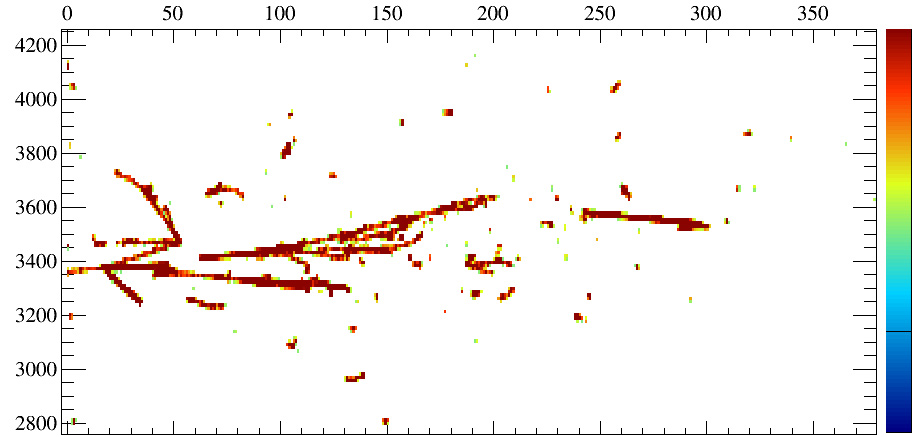
\includegraphics[width=0.45\textwidth]{cnn_1__evd.png}
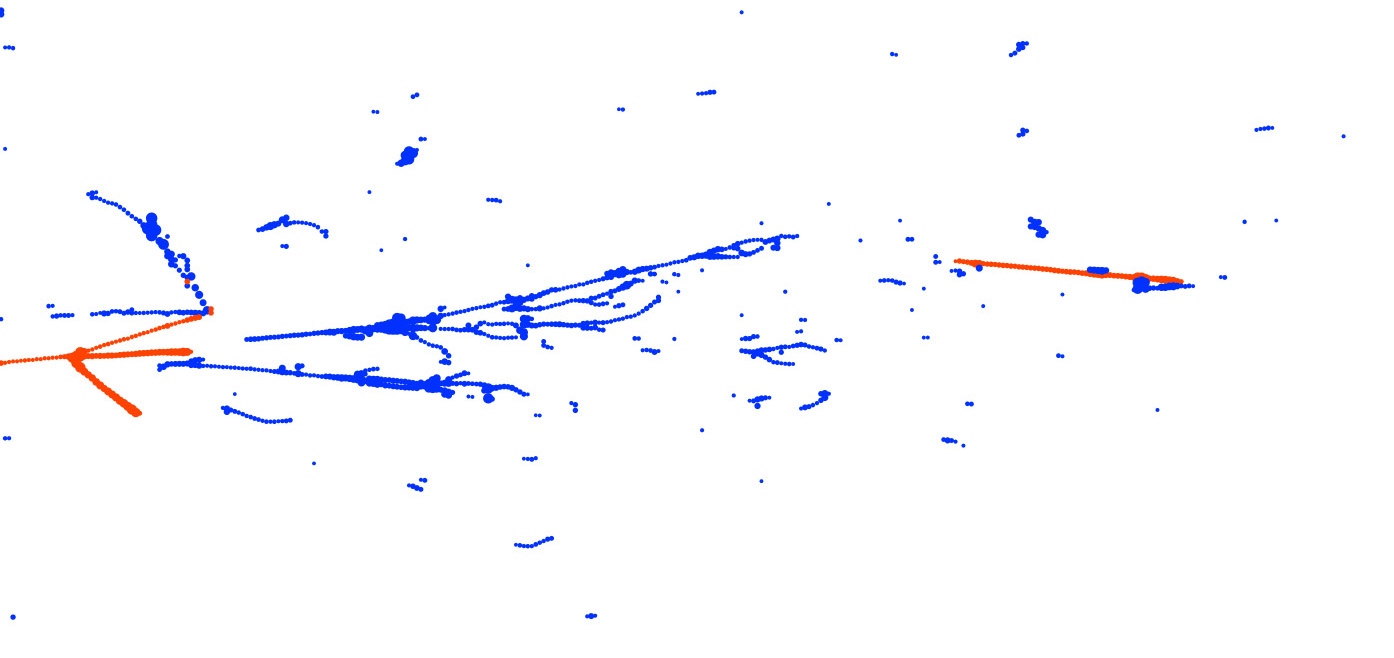
\includegraphics[width=0.45\textwidth]{cnn_2__output_pip2p5GeV_clu_em.png}
\end{cdrfigure}

\begin{cdrfigure}[CNN-based EM selection in pion samples]{cnnemselinsamples}{ADC area
in hits selected with CNN as electromagnetic activity versus ADC area in hits selected
with MC truth information as originating from electron tracks: simulated in ProtoDUNE
geometry events with positive pion in the test beam at momentum 1~GeV$/c$ (left) and
4~GeV$/c$ (right).}
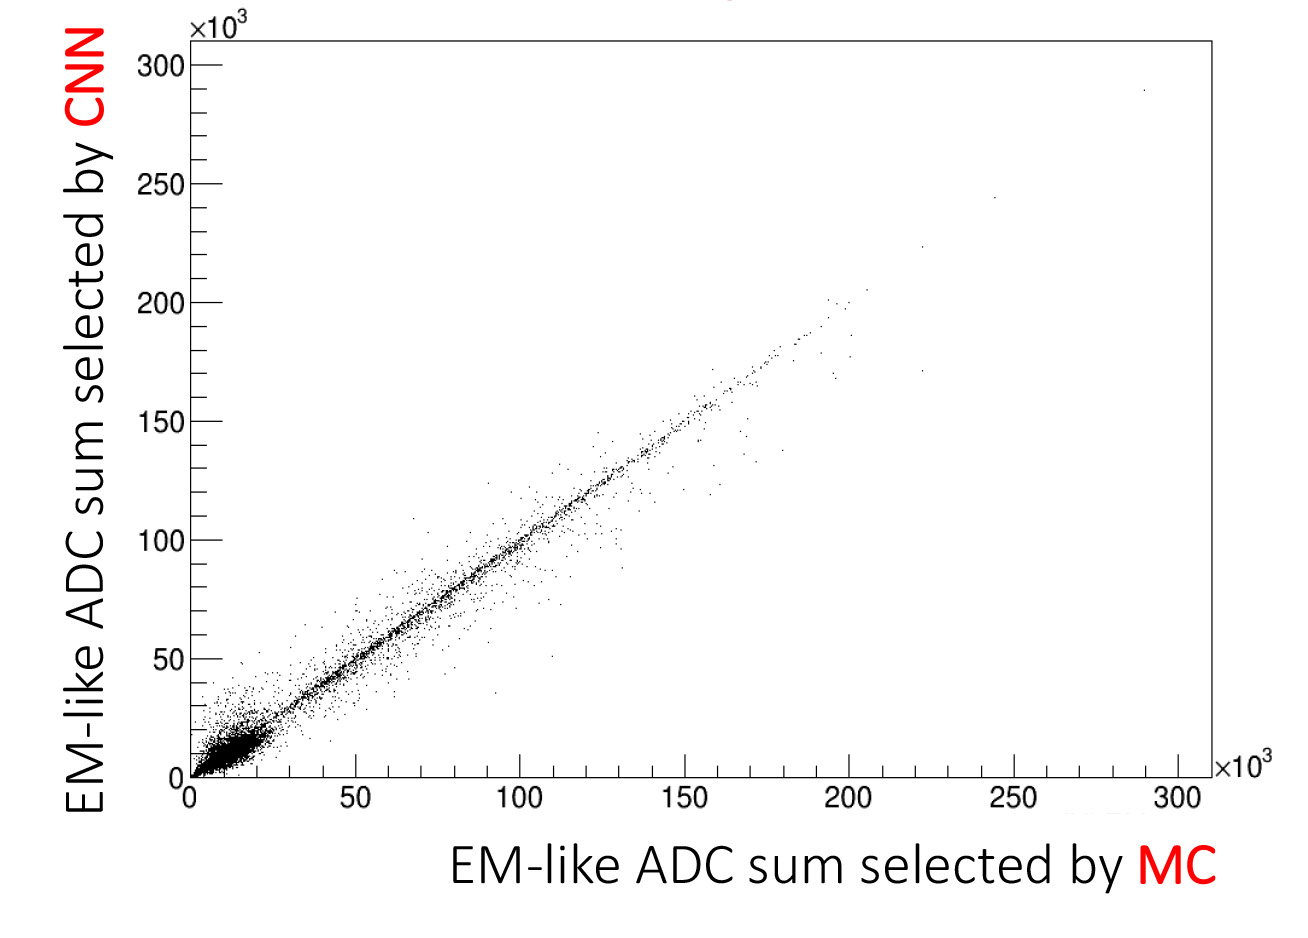
\includegraphics[width=0.45\textwidth]{cnn_3__pi_1GeV.png}
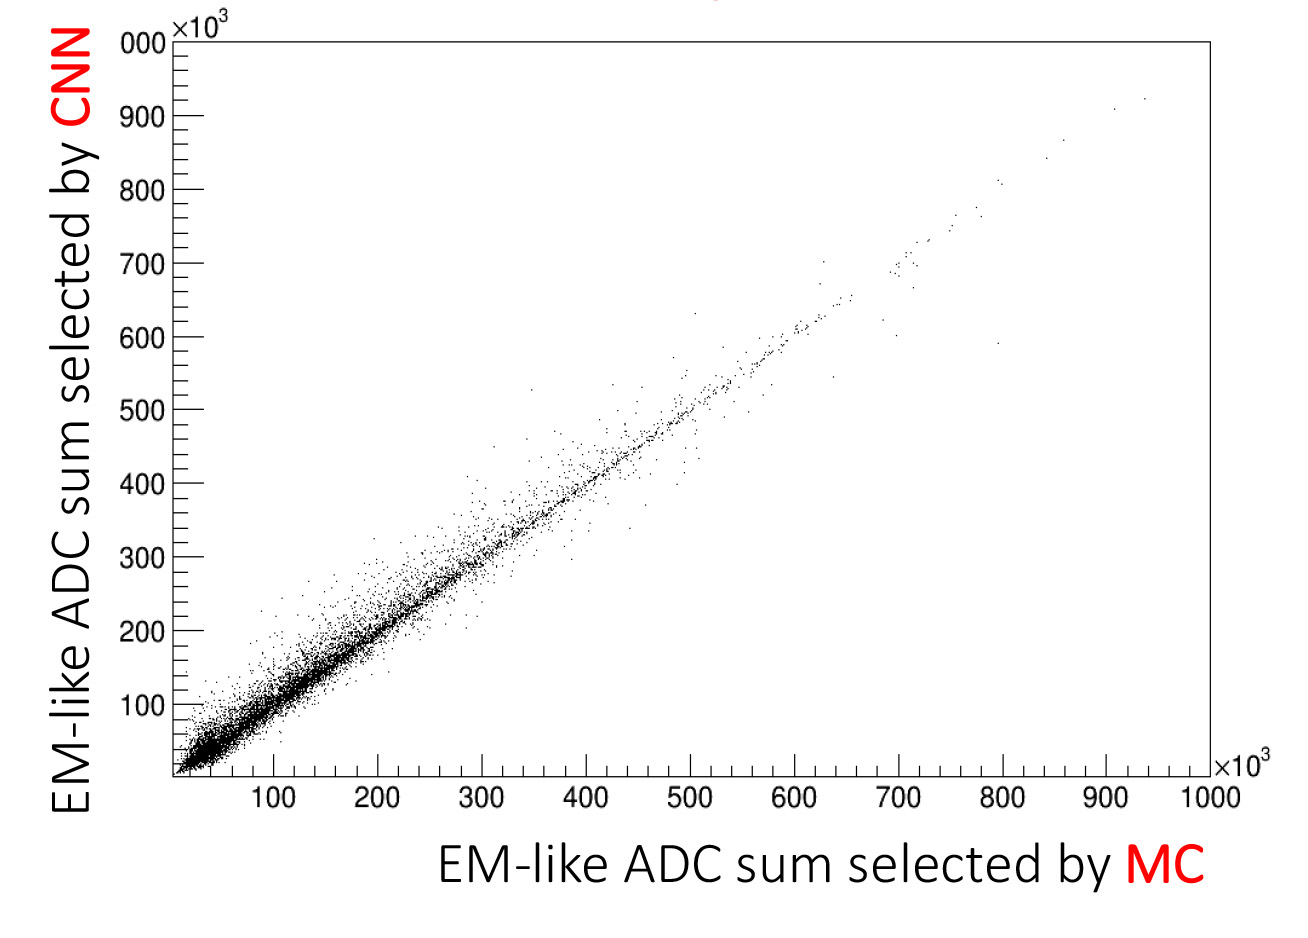
\includegraphics[width=0.45\textwidth]{cnn_4__pi_4GeV.png}
\end{cdrfigure}


%%%%
\subsubsection{EMShower}

The EMShower package~\cite{emshowerpackage} takes the output of the
Blurred Clustering Algorithm and
produces energies, angles, and start positions for 3D showers, as
well as the $dE/dx$ in the initial part of the shower.  Identifying
events with two showers consistent with $\pi^0\rightarrow\gamma\gamma$
decays allows for an \textit{in situ} calibration of the electromagnetic
energy scale as well as the performance of shower identification and
reconstruction for photons that are produced inside the detector.  A
distribution of reconstructed $\pi^0$ masses in Monte Carlo is shown
in Figure~\ref{fig:pizeromass}.

\begin{cdrfigure}[Reconstructed invariant masses of $\pi^0$ candidates in
  MC]{pizeromass}{The reconstructed invariant masses of $\pi^0$ candidates in
  Monte Carlo using the BlurredCluster and EMShower algorithms.}
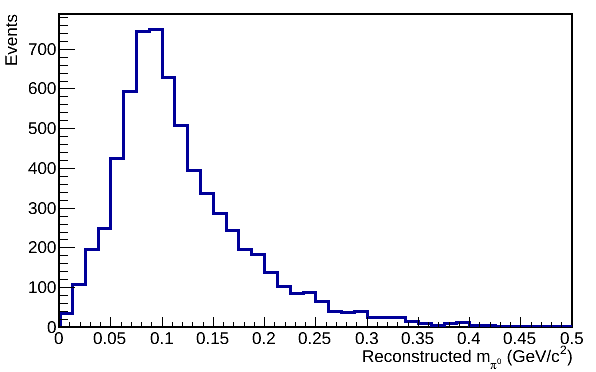
\includegraphics[width=0.8\textwidth]{pizeromass}
\end{cdrfigure}

%%%%
\subsubsection{PANDORA}

The reconstruction framework PANDORA~\cite{Marshall:2015rfa} also works by
building up a 3D picture from 2D
reconstructed objects.  PANDORA is a flexible framework developed for
International Linear Collider (ILC) detector simulation, and provides a convenient way to develop
algorithms for reconstructing particles.  In all, more than 80
algorithms, each targeting a specific topology, have been incorporated
into PANDORA to date.  PANDORA allows multiple reconstruction passes through the data.  
%Multiple passes through reconstructing the data are possible. 
Different criteria for clustering hits into tracks and
showers may be applied when seeking to remove cosmic rays %rather 
than when
identifying signal events.  PANDORA follows a process that clusters hits in 2D,
reconstructs vertices in 3D, reconstructs tracks in 3D,
reconstructs showers in 3D, performs a \textit{mop-up} step in 2D and 3D, and finally performs
full event-building in 3D.


Plots of the efficiency, the completeness, and the  difference between the true and reconstructed
track lengths for single muons with momentum between 300\,MeV and 5\,GeV in the~\pdsp geometry are
shown in Figure~\ref{fig:muonpandoraperf}.  The PANDORA algorithm performs very well, although a small
inefficiency occurs in the current algorithm's ability to match track segments from one APA's drift volume to another.

\begin{cdrfigure}[PANDORA reconstruction, single muons, 300~MeV$/c$ < $p$ < 5~GeV/$c$]{muonpandoraperf}{Performance of the PANDORA reconstruction algorithm for single muons with 
momentum between 300~MeV$/c$ and 5~GeV/$c$.  The top left-hand figure shows the tracking efficiency as a function of
muon momentum, the top right-hand figure shows the distribution of tracking completeness, and the bottom figure shows the
distribution of the difference between the reconstructed muon track length and the true track length.}
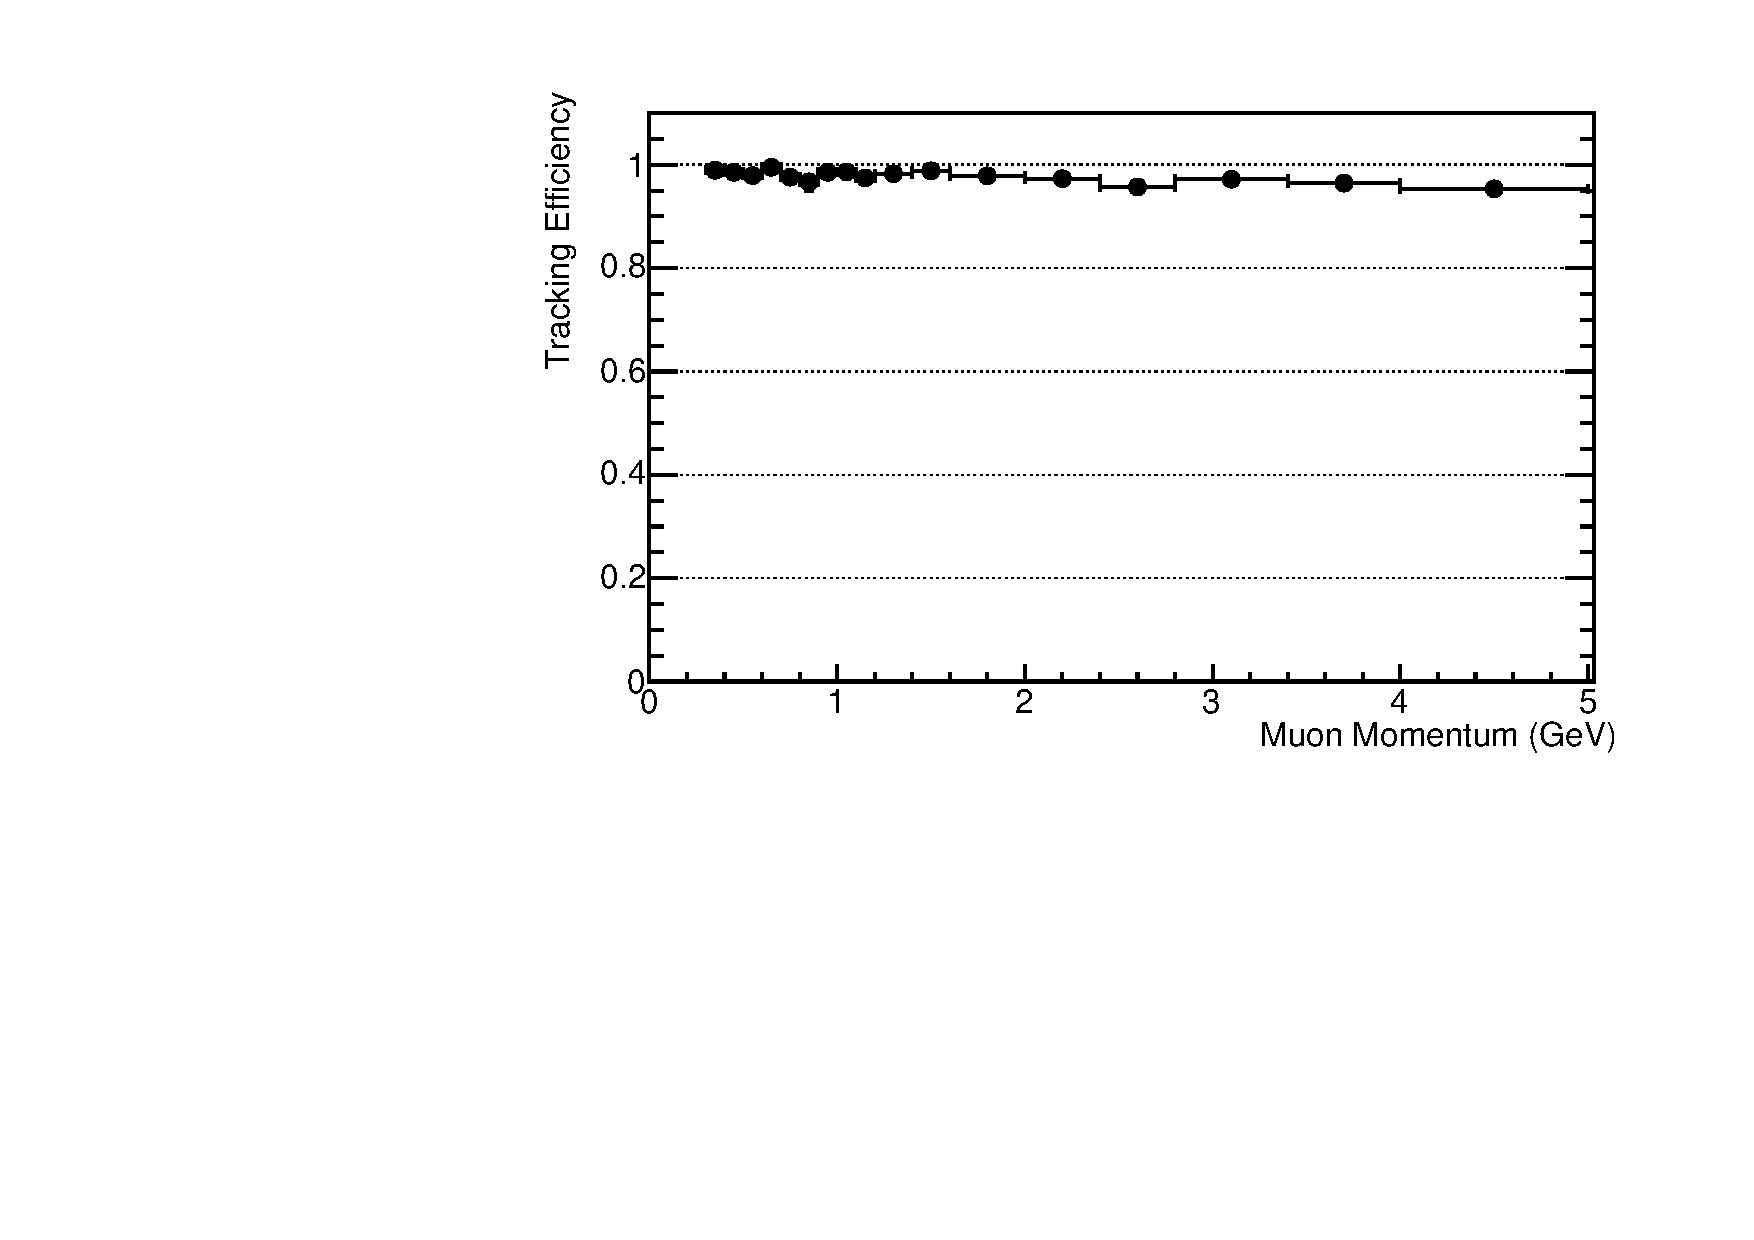
\includegraphics[width=0.45\textwidth]{mu_eff_pandora.pdf}
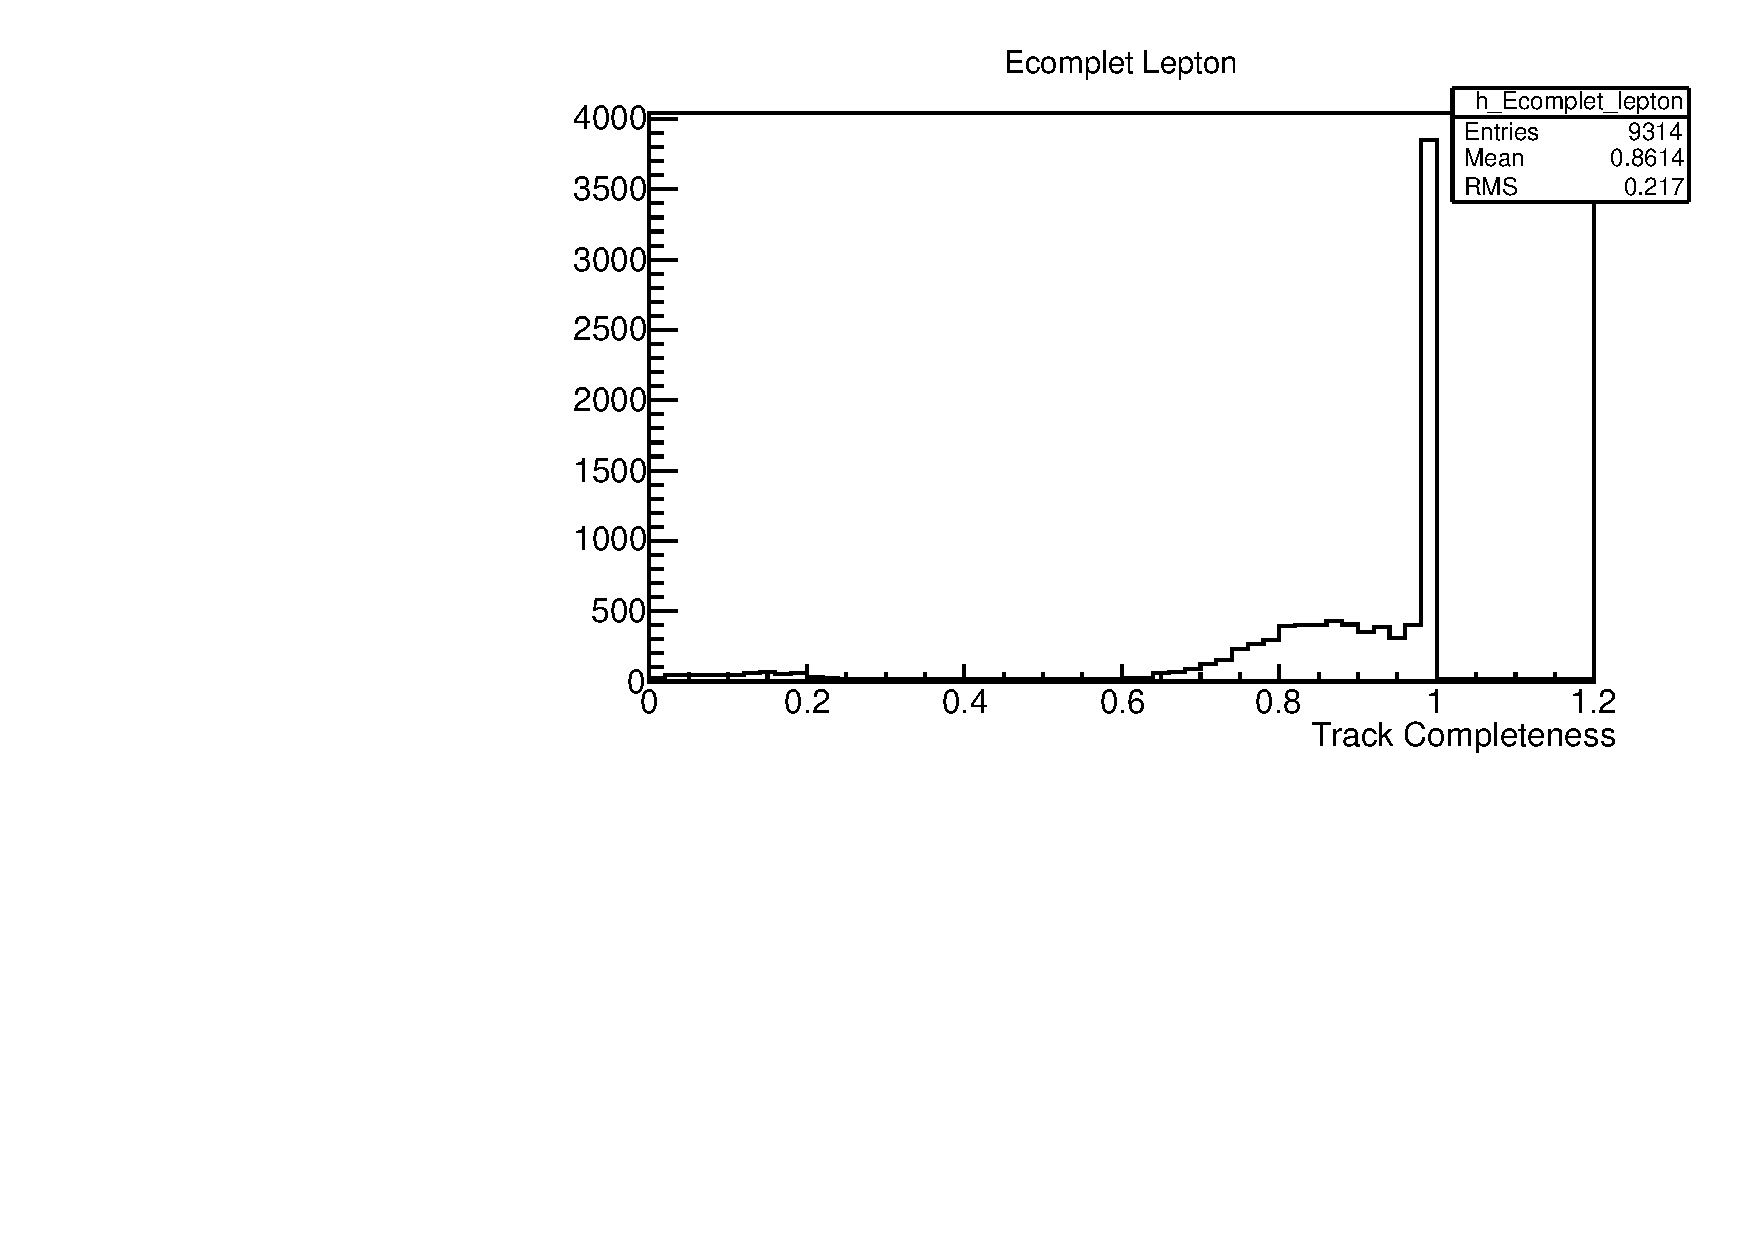
\includegraphics[width=0.45\textwidth]{trk_completeness_pandora.pdf}
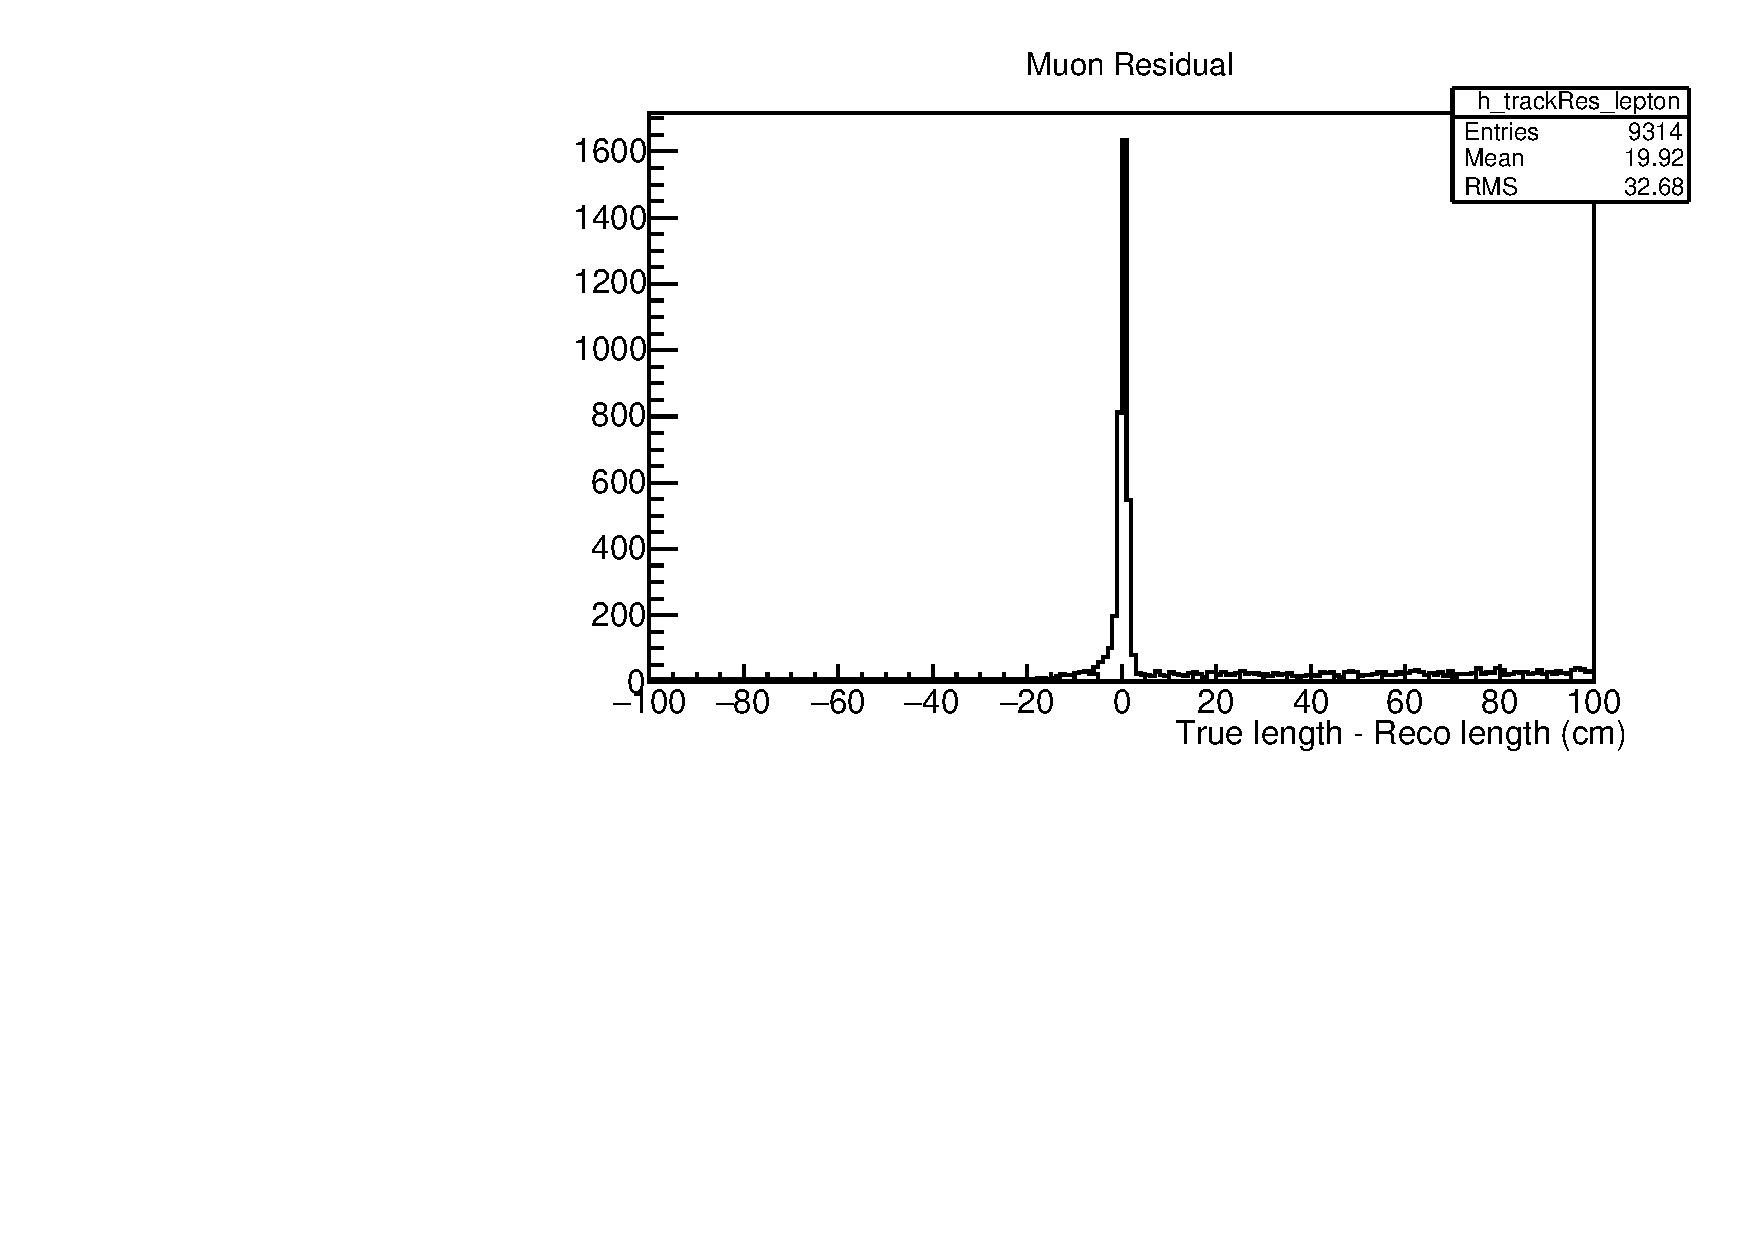
\includegraphics[width=0.45\textwidth]{mu_res_pandora.pdf}
\end{cdrfigure}


%%%%
\subsubsection{PMA}

Another approach to 3D reconstruction in LArTPC detectors is referred to as the \textit{Projection Matching Algorithm
(PMA)}~\cite{pma_algorithm}. PMA was primarily developed as a technique for 3D reconstruction
of individual particle trajectories (trajectory fits). 
Instead of
building up a 3D hypothesis from 2D clusters, it starts with the 3D hypothesis and compares
the 2D projection of the predicted trajectory of a particle with the observed data. Association
of hits between the 2D planes is not needed in this approach, improving its performance in
problematic cases, such as isochronous and short tracks.

PMA can take as input the output from different pattern recognition algorithms, from
LineCluster~\cite{linecluster} to WireCell (described below).  Because these 2D algorithms
are run on each 2D projection independently, and because of detector defects,
clusters from  particles may be broken
into several smaller pieces, fractions of 2D clusters may be missing,
and clusters obtained from complementary projections are not guaranteed to cover corresponding
sections of trajectories. Such behavior is expected since ambiguous 
trajectories can be resolved only if the information from multiple 2D projections is used.
PMA performs higher-level pattern recognition using as input clustering information from all
projections in order to search for the best matching combinations of clusters. The algorithm
also attempts to correct hit-to-cluster assignments using properties of 3D reconstructed objects.

Plots of the efficiency, the completeness, and the  difference between the true and reconstructed
track lengths for single muons with momentum between 300\,MeV and 5\,GeV in the~\pdsp geometry are
shown in Figure~\ref{fig:muonpmaperf}.  

\begin{cdrfigure}[PMA reconstruction, single muons, 300\,MeV/c < $p$ < 5\,GeV/c]{muonpmaperf}{Performance of the PMA reconstruction algorithm for single muons with 
momentum between 300~MeV/c and 5~GeV/c.  The left-hand figure shows the tracking efficiency as a function of
muon momentum, the middle figure shows the distribution of tracking completeness, and the right-hand figure shows the
distribution of the difference between the reconstructed muon track length and the true track length.}
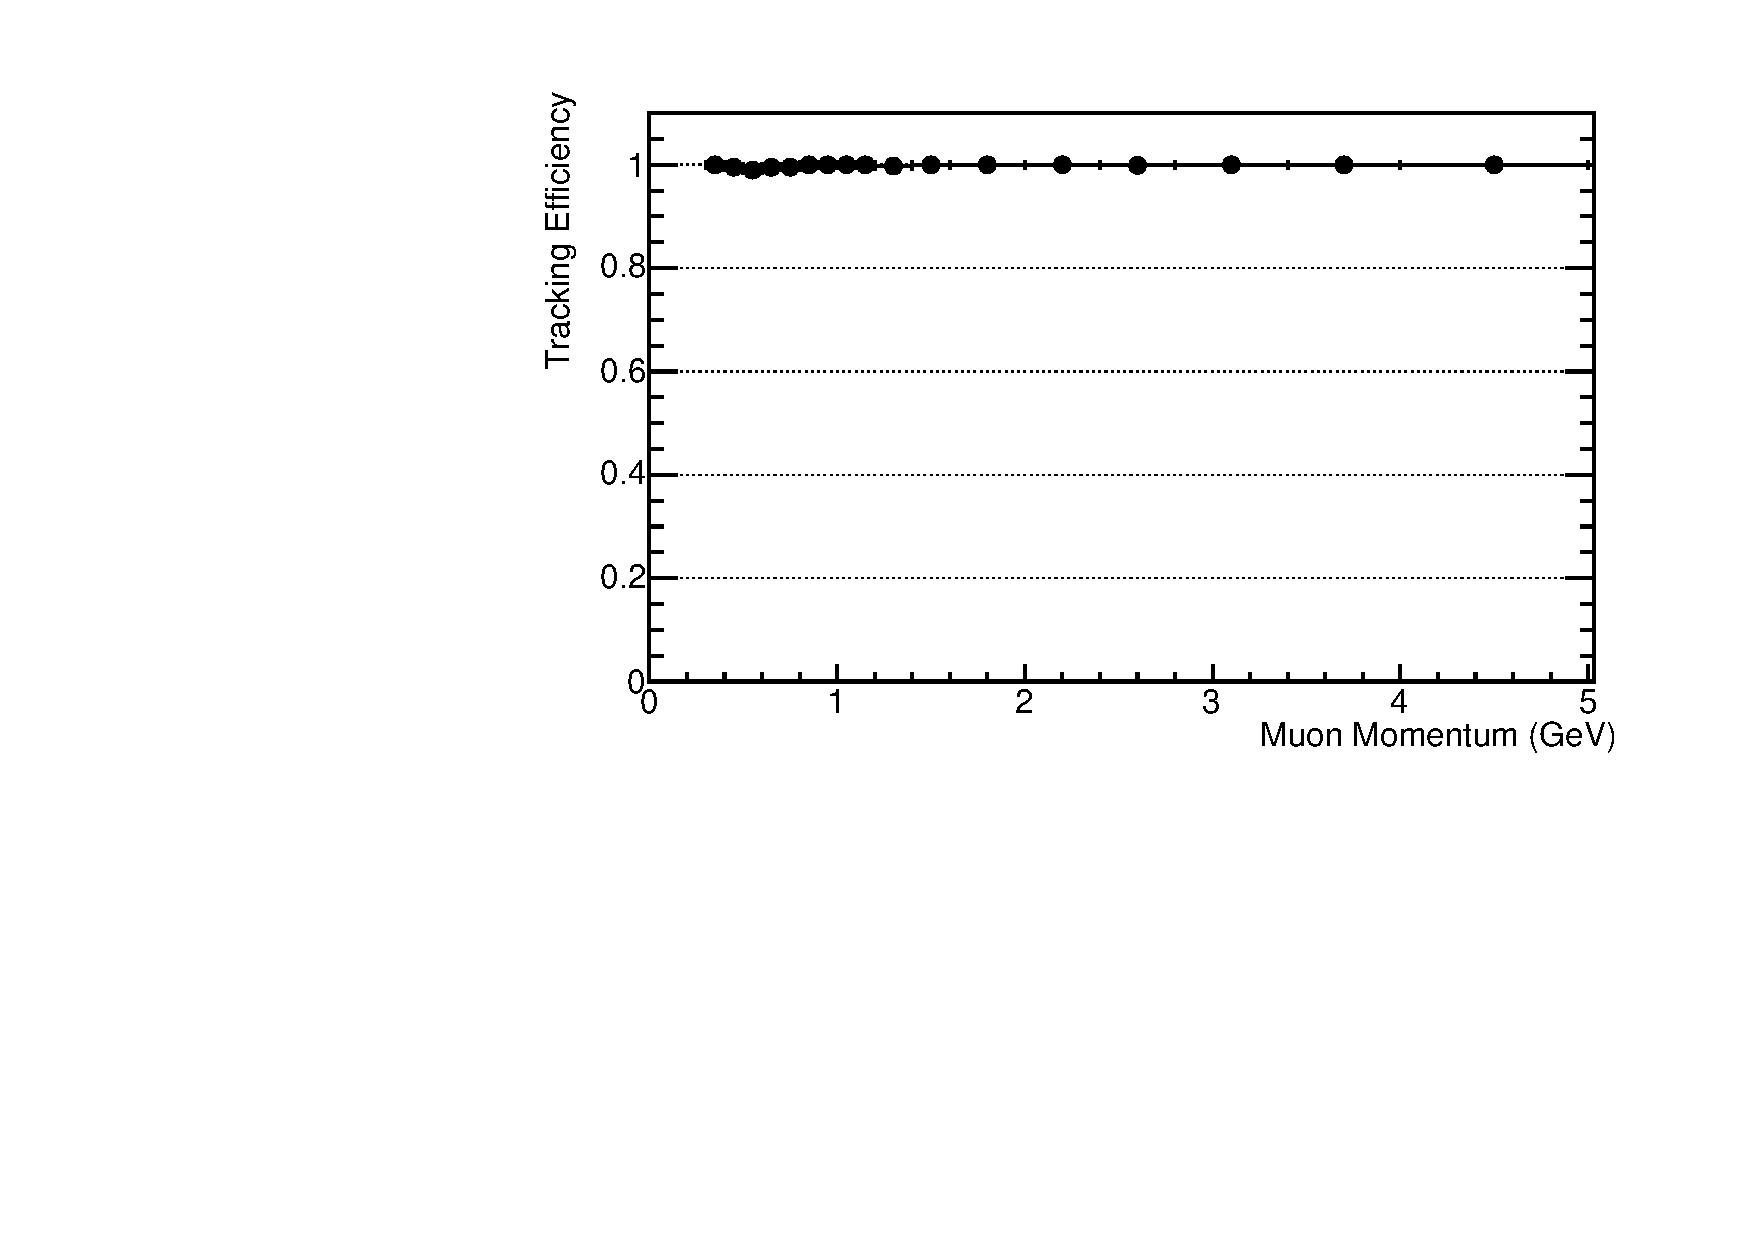
\includegraphics[width=0.45\textwidth]{mu_eff_pmtrack.pdf}
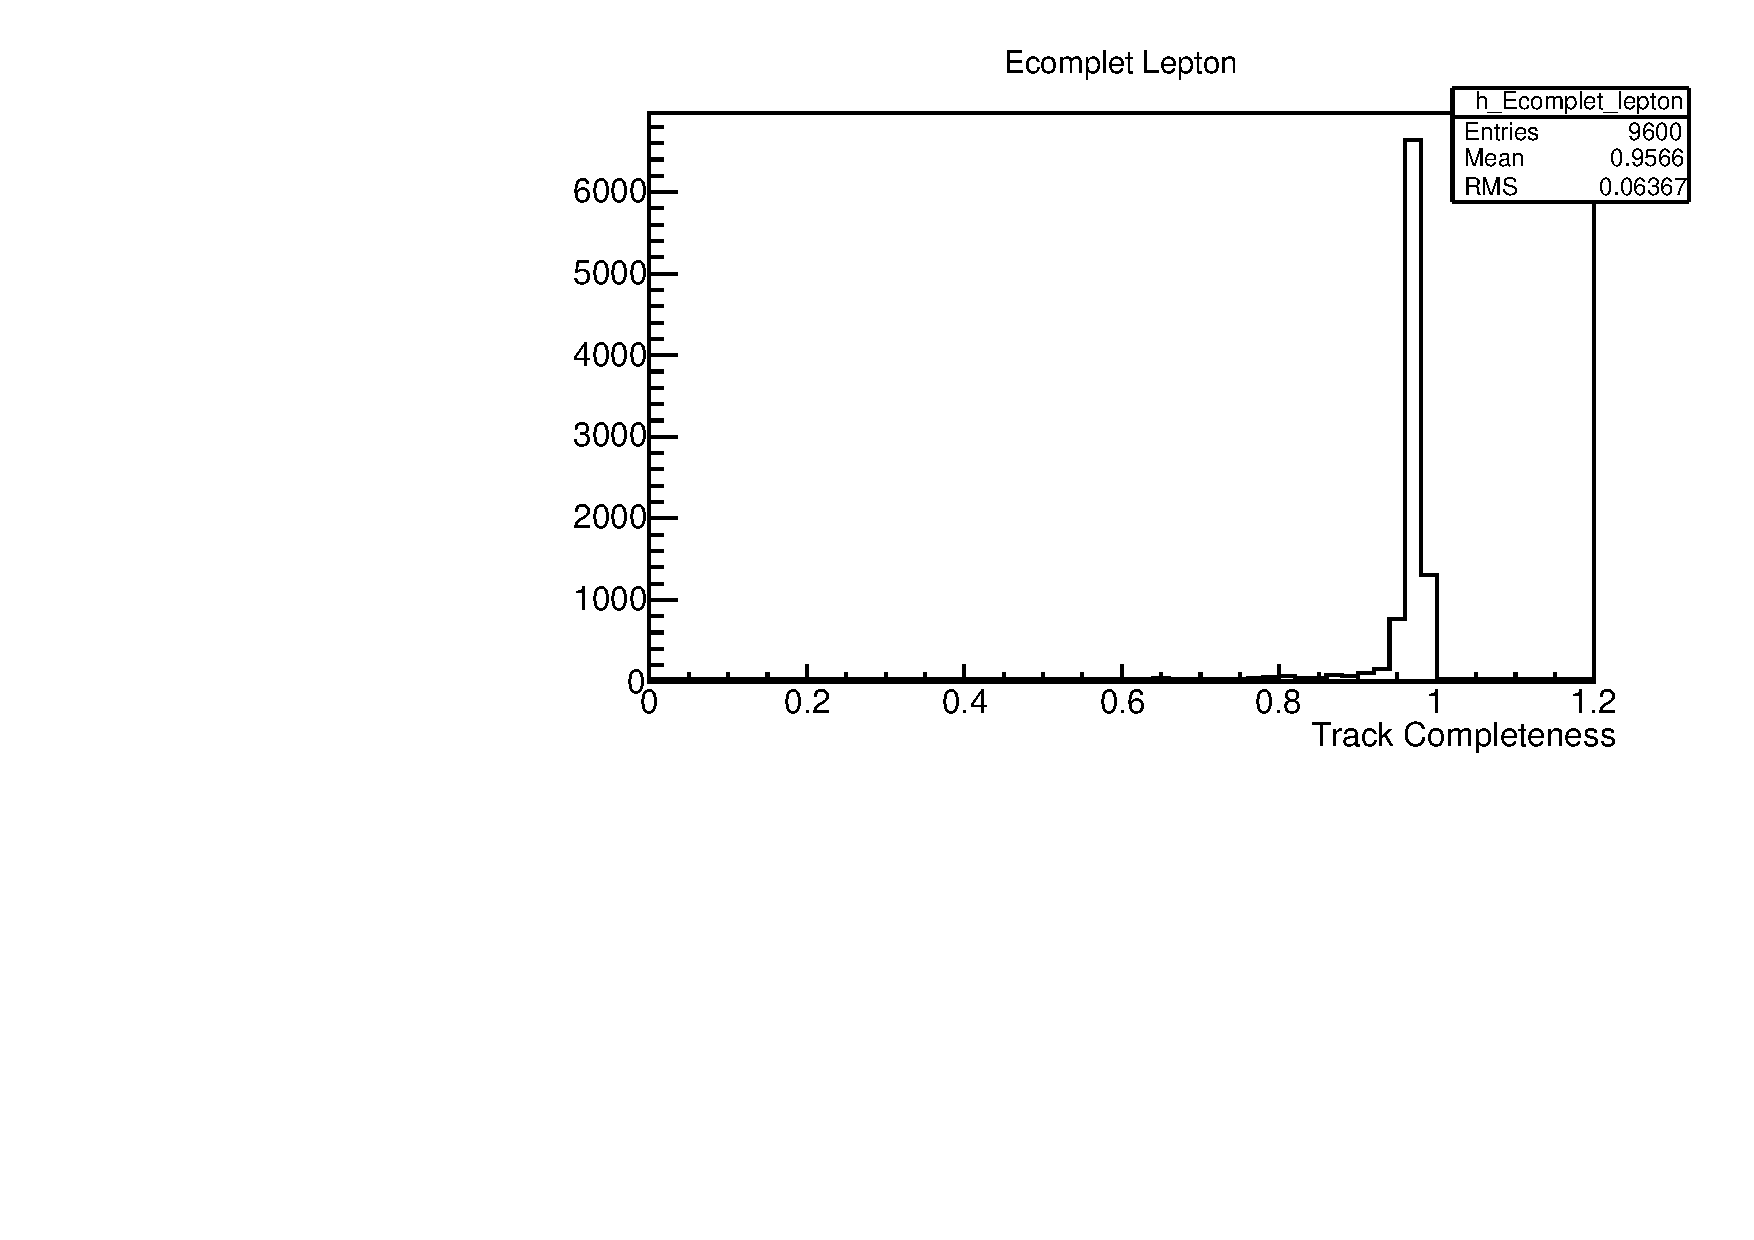
\includegraphics[width=0.45\textwidth]{trk_completeness_pmtrack.pdf}
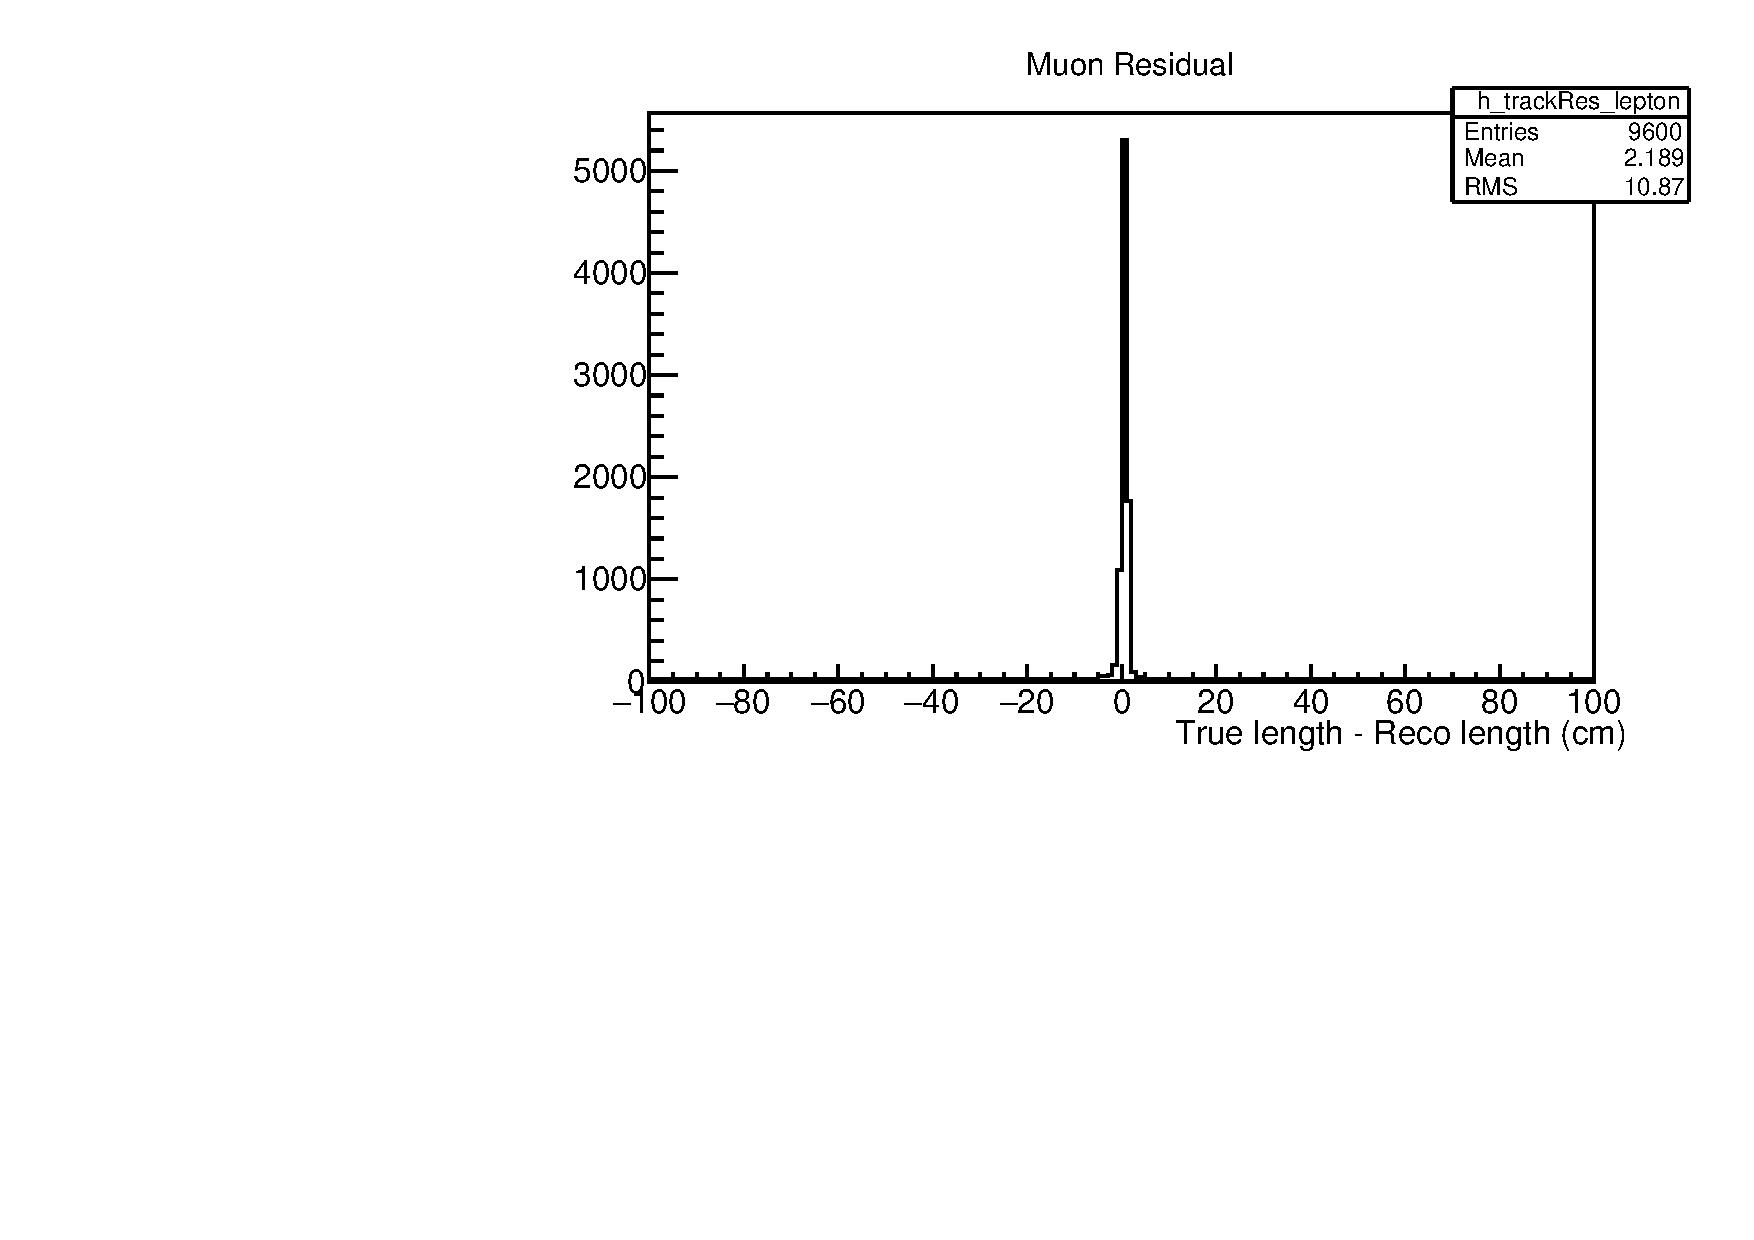
\includegraphics[width=0.45\textwidth]{mu_res_pmtrack.pdf}
\end{cdrfigure}

PMA has been used successfully in \pdsp to reconstruct simulated beam particles and cosmic muons~\cite{pma_cosmic_mu}. In order to illustrate the performance of the entire reconstruction chain,
Figure~\ref{fig:PMApioninteraction} shows the spatial resolution of the interaction vertex with neutral pion
production appearing in the 2-GeV/c $\pi^+$ sample.
The resolution is found to be 0.6\,cm in this study.
A similar resolution is obtained for the reconstruction
of inelastic interaction vertices in the 2-GeV/c proton sample. 


Figures~\ref{fig:PMAproton2gevc}
and~\ref{fig:PMAcosmics} show examples of reconstruction of a 2-GeV/c proton in the test beam and
cosmic-ray muons, respectively.

\begin{cdrfigure}[Vertex resolution for
  inelastic interaction of $\pi^\pm$ on Ar where a $\pi^0$ is produced]{PMApioninteraction}{Vertex position resolution in cm in $x$, $y$, and $z$ and 3D for the
  inelastic interaction of charged pions on liquid argon nuclei in events in which a $\pi^0$ is produced, in
  \pdsp, using the PMA algorithm.}
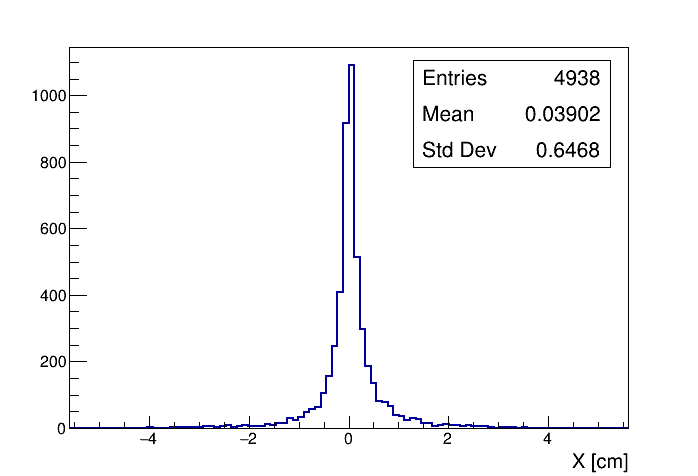
\includegraphics[width=0.45\textwidth]{pi0_vtx_dx.png}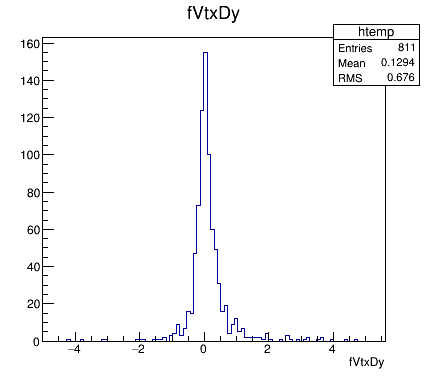
\includegraphics[width=0.45\textwidth]{figures/pi0_vtx_dy.png}
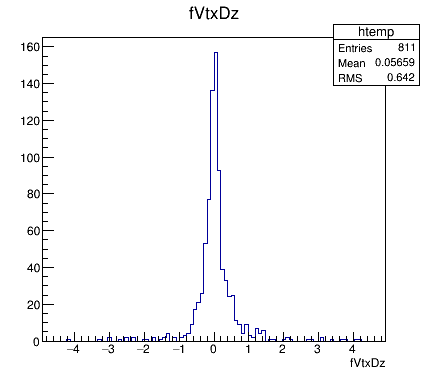
\includegraphics[width=0.45\textwidth]{pi0_vtx_dz.png}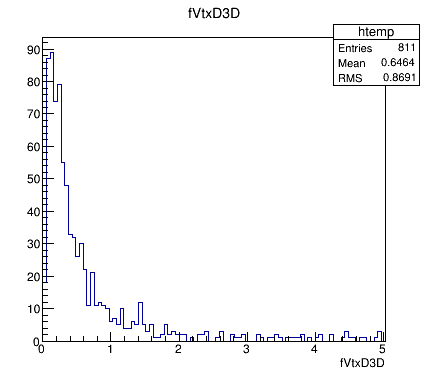
\includegraphics[width=0.45\textwidth]{figures/pi0_vtx3d.png}
\end{cdrfigure}


\begin{cdrfigure}[Reconstructed event of simulated proton with initial momentum 2\,GeV/c]{PMAproton2gevc}{Example of reconstructed event of simulated proton with initial momentum 2\,GeV/c (reconstruction algorithms: gaushit, Line Cluster and PMA).}
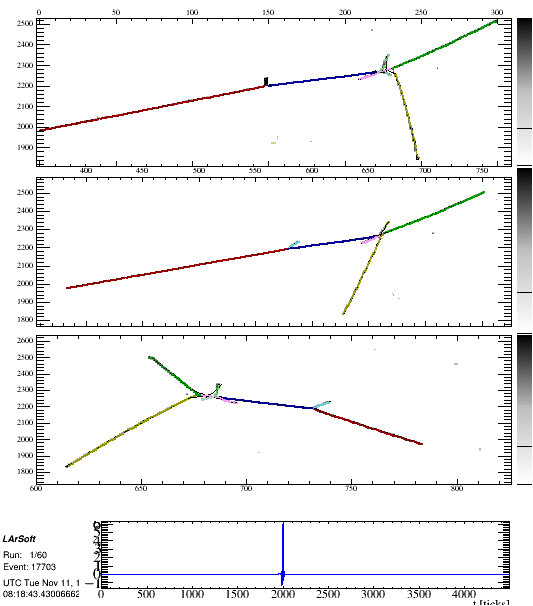
\includegraphics[width=0.45\textwidth]{figures/evdtwqproj117703.png}
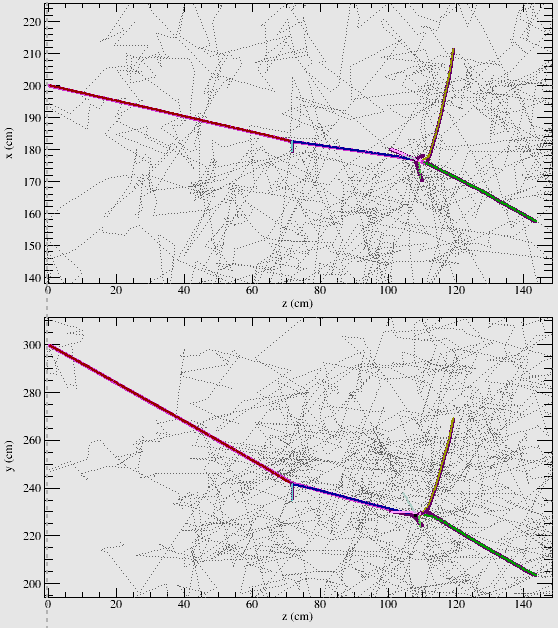
\includegraphics[width=0.45\textwidth]{figures/evdlarortho3d117703.png}
\end{cdrfigure}
\begin{cdrfigure}[Example of reconstructed cosmic muons in \pdsp]{PMAcosmics}{Example of reconstructed cosmic muons using gaushit, Line Cluster and PMA.}
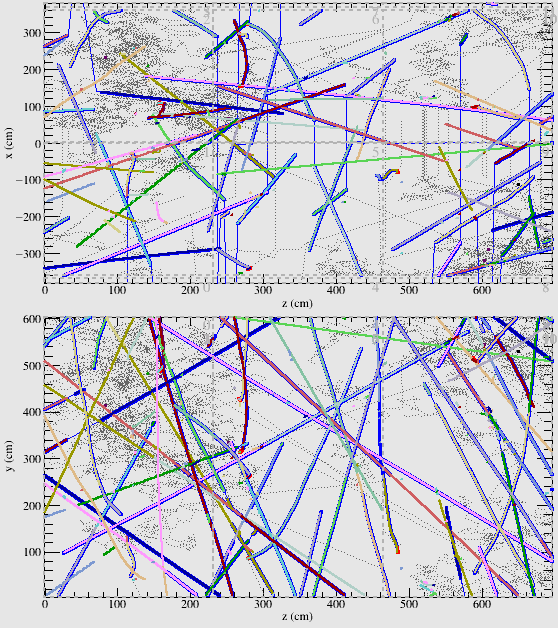
\includegraphics[width=0.45\textwidth]{figures/evdlarortho3d11302.png}
\end{cdrfigure}



%%%%
\subsubsection{WireCell}

WireCell~\cite{wire-cell}, a new reconstruction method under development, adopts a very different approach from the aforementioned algorithms .
Instead of performing pattern recognition directly on each of the 2D views (drift 
time versus wire number), the first step of the WireCell reconstruction is to 
perform 3D imaging with time, geometry, and charge information. 
The algorithm takes advantage of this % timing, geometry, and charge 
information to suppress the effects of electronic noise.
%
Often, noise will lead to a fluctuation in a waveform which may be
large enough to mimic a signal.  The algorithm combats this by
requiring any potential signal to be consistent across multiple wires,
given their geometry, in their charge across time.  Many of the
fluctuations due to noise will fail this consistency requirement and
be rejected while true signal will satisfy it.
%
Use of the charge and time information in this manner takes advantage of the fact that in a LArTPC with induction planes,
each of the wire planes, in principle, detects the same ionization electrons as the other planes. 
Figure~\ref{fig:quality} shows an example of the improvement of WireCell 3D imaging
over the more traditional approach. 

%However, 
The suppression of the electronic noise comes at the cost of more
sensitivity to hit inefficiencies from dead channels or the signal processing steps.
 Since the track and shower hypotheses
are not used, the 3D imaging works for any event topology. 
Pattern recognition is needed to identify 
the content of these 3D images. Figure~\ref{fig:tracking2} shows the 
performance of the currently available 3D pattern recognition in
WireCell. For the long track going close to parallel to the wire plane, the reconstructed
track shows a zig-zag behavior. This is due to the current lack of a fine track-fitting algorithm
that is expected to be added in the near future. 
Further developments of the WireCell pattern recognition algorithms
are needed before meaningful physics quantities can be calculated.
%
%% Wire-Cell Imaging
\begin{cdrfigure}[Comparison of imaging recon
qualities with and without charge information]{quality}{Comparison of imaging reconstruction 
qualities with and without the charge information. }
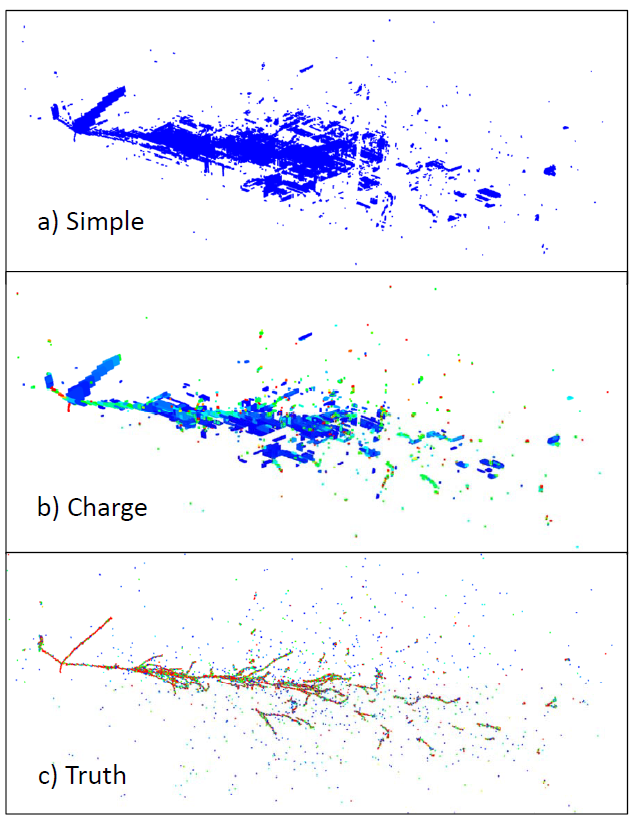
\includegraphics[width=0.5\textwidth]{quality.png}
\end{cdrfigure}
%
%
%% Wire-Cell 3D pattern recognition
\begin{cdrfigure}[Reconstructed image for one neutrino interaction event; comparison to MC]{tracking2}{The reconstructed image is shown 
on the left panel for one neutrino interaction event. The image 
was passed through the 3D pattern recognition program with tracks 
identified (middle panel). The identified pattern is compared 
with Monte-Carlo truth in the right panel. The zig-zag line in the right 
panel is the identified track.  More sophisticated track-fitting algorithms, to be added in the future,
will improve the track reconstruction.}
 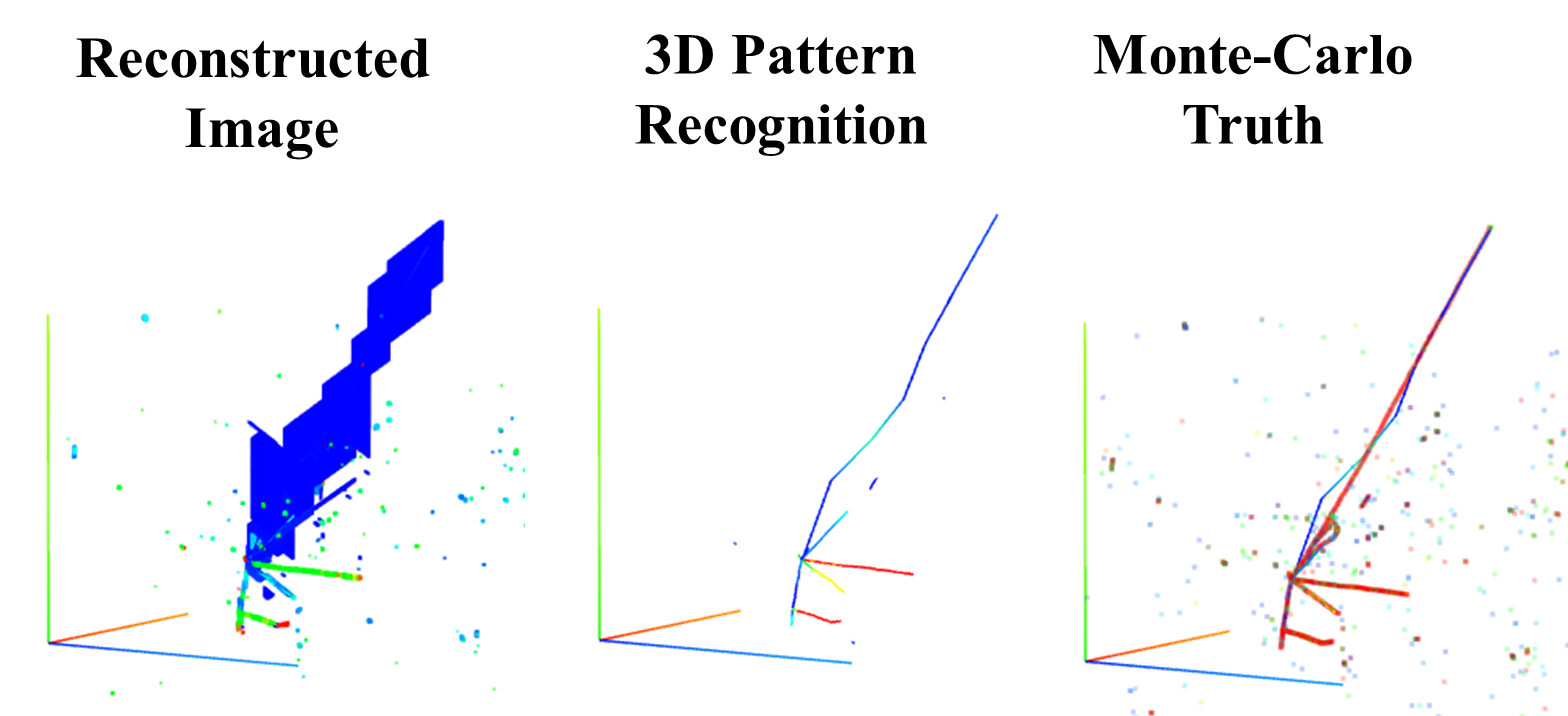
\includegraphics[width=0.9\textwidth]{Tracking_2.png}
\end{cdrfigure}

